


\tikzset{every picture/.style={line width=0.75pt}} %set default line width to 0.75pt        

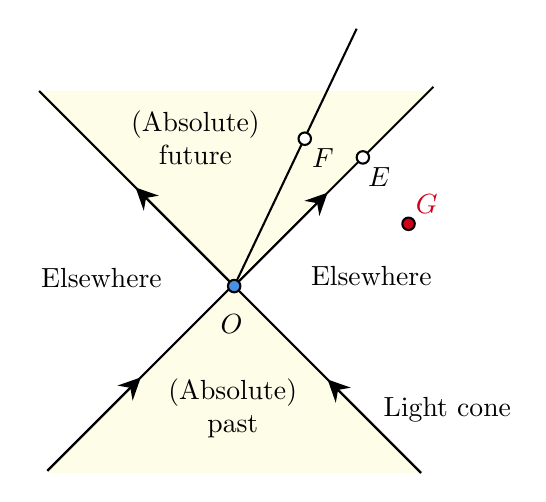
\begin{tikzpicture}[x=0.75pt,y=0.75pt,yscale=-1,xscale=1]
%uncomment if require: \path (0,236); %set diagram left start at 0, and has height of 236

%Shape: Triangle [id:dp5873969882948538] 
\draw  [draw opacity=0][fill={rgb, 255:red, 248; green, 231; blue, 28 }  ,fill opacity=0.1 ] (116,131) -- (206,221) -- (26,221) -- cycle ;
%Shape: Triangle [id:dp3732778658861451] 
\draw  [draw opacity=0][fill={rgb, 255:red, 248; green, 231; blue, 28 }  ,fill opacity=0.1 ] (116,131) -- (212,37) -- (22,37) -- cycle ;
%Straight Lines [id:da06512352307651148] 
\draw [color={rgb, 255:red, 0; green, 0; blue, 0 }  ,draw opacity=1 ]   (117,130) -- (27,220) ;
%Straight Lines [id:da078661412644073] 
\draw [color={rgb, 255:red, 0; green, 0; blue, 0 }  ,draw opacity=1 ]   (23,37) -- (117,131) ;
%Straight Lines [id:da9236403245545768] 
\draw [color={rgb, 255:red, 0; green, 0; blue, 0 }  ,draw opacity=1 ]   (117,131) -- (213,35) ;
%Straight Lines [id:da6706956851866872] 
\draw [color={rgb, 255:red, 0; green, 0; blue, 0 }  ,draw opacity=1 ]   (117,131) -- (207,221) ;
%Straight Lines [id:da49716251260450606] 
\draw [color={rgb, 255:red, 0; green, 0; blue, 0 }  ,draw opacity=1 ]   (27,220) -- (69.88,177.12) ;
\draw [shift={(72,175)}, rotate = 135] [fill={rgb, 255:red, 0; green, 0; blue, 0 }  ,fill opacity=1 ][line width=0.08]  [draw opacity=0] (10.72,-5.15) -- (0,0) -- (10.72,5.15) -- (7.12,0) -- cycle    ;
%Straight Lines [id:da689124165646404] 
\draw [color={rgb, 255:red, 0; green, 0; blue, 0 }  ,draw opacity=1 ]   (117,131) -- (71.62,85.62) ;
\draw [shift={(69.5,83.5)}, rotate = 45] [fill={rgb, 255:red, 0; green, 0; blue, 0 }  ,fill opacity=1 ][line width=0.08]  [draw opacity=0] (10.72,-5.15) -- (0,0) -- (10.72,5.15) -- (7.12,0) -- cycle    ;
%Straight Lines [id:da6402889619991756] 
\draw [color={rgb, 255:red, 0; green, 0; blue, 0 }  ,draw opacity=1 ]   (117,131) -- (159.88,88.12) ;
\draw [shift={(162,86)}, rotate = 135] [fill={rgb, 255:red, 0; green, 0; blue, 0 }  ,fill opacity=1 ][line width=0.08]  [draw opacity=0] (10.72,-5.15) -- (0,0) -- (10.72,5.15) -- (7.12,0) -- cycle    ;
%Straight Lines [id:da9661258357237661] 
\draw [color={rgb, 255:red, 0; green, 0; blue, 0 }  ,draw opacity=1 ]   (117,131) -- (176,7) ;
%Shape: Circle [id:dp11639370816389172] 
\draw  [color={rgb, 255:red, 0; green, 0; blue, 0 }  ,draw opacity=1 ][fill={rgb, 255:red, 74; green, 144; blue, 226 }  ,fill opacity=1 ] (114,131) .. controls (114,129.34) and (115.34,128) .. (117,128) .. controls (118.66,128) and (120,129.34) .. (120,131) .. controls (120,132.66) and (118.66,134) .. (117,134) .. controls (115.34,134) and (114,132.66) .. (114,131) -- cycle ;
%Shape: Circle [id:dp28922251251628683] 
\draw  [color={rgb, 255:red, 0; green, 0; blue, 0 }  ,draw opacity=1 ][fill={rgb, 255:red, 255; green, 255; blue, 255 }  ,fill opacity=1 ] (148,60) .. controls (148,58.34) and (149.34,57) .. (151,57) .. controls (152.66,57) and (154,58.34) .. (154,60) .. controls (154,61.66) and (152.66,63) .. (151,63) .. controls (149.34,63) and (148,61.66) .. (148,60) -- cycle ;
%Shape: Circle [id:dp952901887366238] 
\draw  [color={rgb, 255:red, 0; green, 0; blue, 0 }  ,draw opacity=1 ][fill={rgb, 255:red, 255; green, 255; blue, 255 }  ,fill opacity=1 ] (176,69) .. controls (176,67.34) and (177.34,66) .. (179,66) .. controls (180.66,66) and (182,67.34) .. (182,69) .. controls (182,70.66) and (180.66,72) .. (179,72) .. controls (177.34,72) and (176,70.66) .. (176,69) -- cycle ;
%Shape: Circle [id:dp5674228873323357] 
\draw  [color={rgb, 255:red, 0; green, 0; blue, 0 }  ,draw opacity=1 ][fill={rgb, 255:red, 208; green, 2; blue, 27 }  ,fill opacity=1 ] (198,101) .. controls (198,99.34) and (199.34,98) .. (201,98) .. controls (202.66,98) and (204,99.34) .. (204,101) .. controls (204,102.66) and (202.66,104) .. (201,104) .. controls (199.34,104) and (198,102.66) .. (198,101) -- cycle ;
%Straight Lines [id:da1677136345722059] 
\draw [color={rgb, 255:red, 0; green, 0; blue, 0 }  ,draw opacity=1 ]   (207,221) -- (164.12,178.12) ;
\draw [shift={(162,176)}, rotate = 45] [fill={rgb, 255:red, 0; green, 0; blue, 0 }  ,fill opacity=1 ][line width=0.08]  [draw opacity=0] (10.72,-5.15) -- (0,0) -- (10.72,5.15) -- (7.12,0) -- cycle    ;

% Text Node
\draw (64,45) node [anchor=north west][inner sep=0.75pt]   [align=left] {\begin{minipage}[lt]{49.21pt}\setlength\topsep{0pt}
\begin{center}
(Absolute)\\future
\end{center}

\end{minipage}};
% Text Node
\draw (82,174) node [anchor=north west][inner sep=0.75pt]   [align=left] {\begin{minipage}[lt]{49.21pt}\setlength\topsep{0pt}
\begin{center}
(Absolute)\\past
\end{center}

\end{minipage}};
% Text Node
\draw (148,120) node [anchor=north west][inner sep=0.75pt]   [align=left] {\begin{minipage}[lt]{50.35pt}\setlength\topsep{0pt}
\begin{center}
Elsewhere
\end{center}

\end{minipage}};
% Text Node
\draw (18,121) node [anchor=north west][inner sep=0.75pt]   [align=left] {\begin{minipage}[lt]{50.35pt}\setlength\topsep{0pt}
\begin{center}
Elsewhere
\end{center}

\end{minipage}};
% Text Node
\draw (185,183) node [anchor=north west][inner sep=0.75pt]  [color={rgb, 255:red, 0; green, 0; blue, 0 }  ,opacity=1 ] [align=left] {\begin{minipage}[lt]{49.79pt}\setlength\topsep{0pt}
\begin{center}
Light cone
\end{center}

\end{minipage}};
% Text Node
\draw (153,63.4) node [anchor=north west][inner sep=0.75pt]  [color={rgb, 255:red, 0; green, 0; blue, 0 }  ,opacity=1 ]  {$F$};
% Text Node
\draw (180,72.4) node [anchor=north west][inner sep=0.75pt]    {$E$};
% Text Node
\draw (203,97.6) node [anchor=south west] [inner sep=0.75pt]  [color={rgb, 255:red, 208; green, 2; blue, 27 }  ,opacity=1 ]  {$G$};
% Text Node
\draw (109,143.4) node [anchor=north west][inner sep=0.75pt]    {$O$};


\end{tikzpicture}